\begin{figure}[htbp]
  \centering
  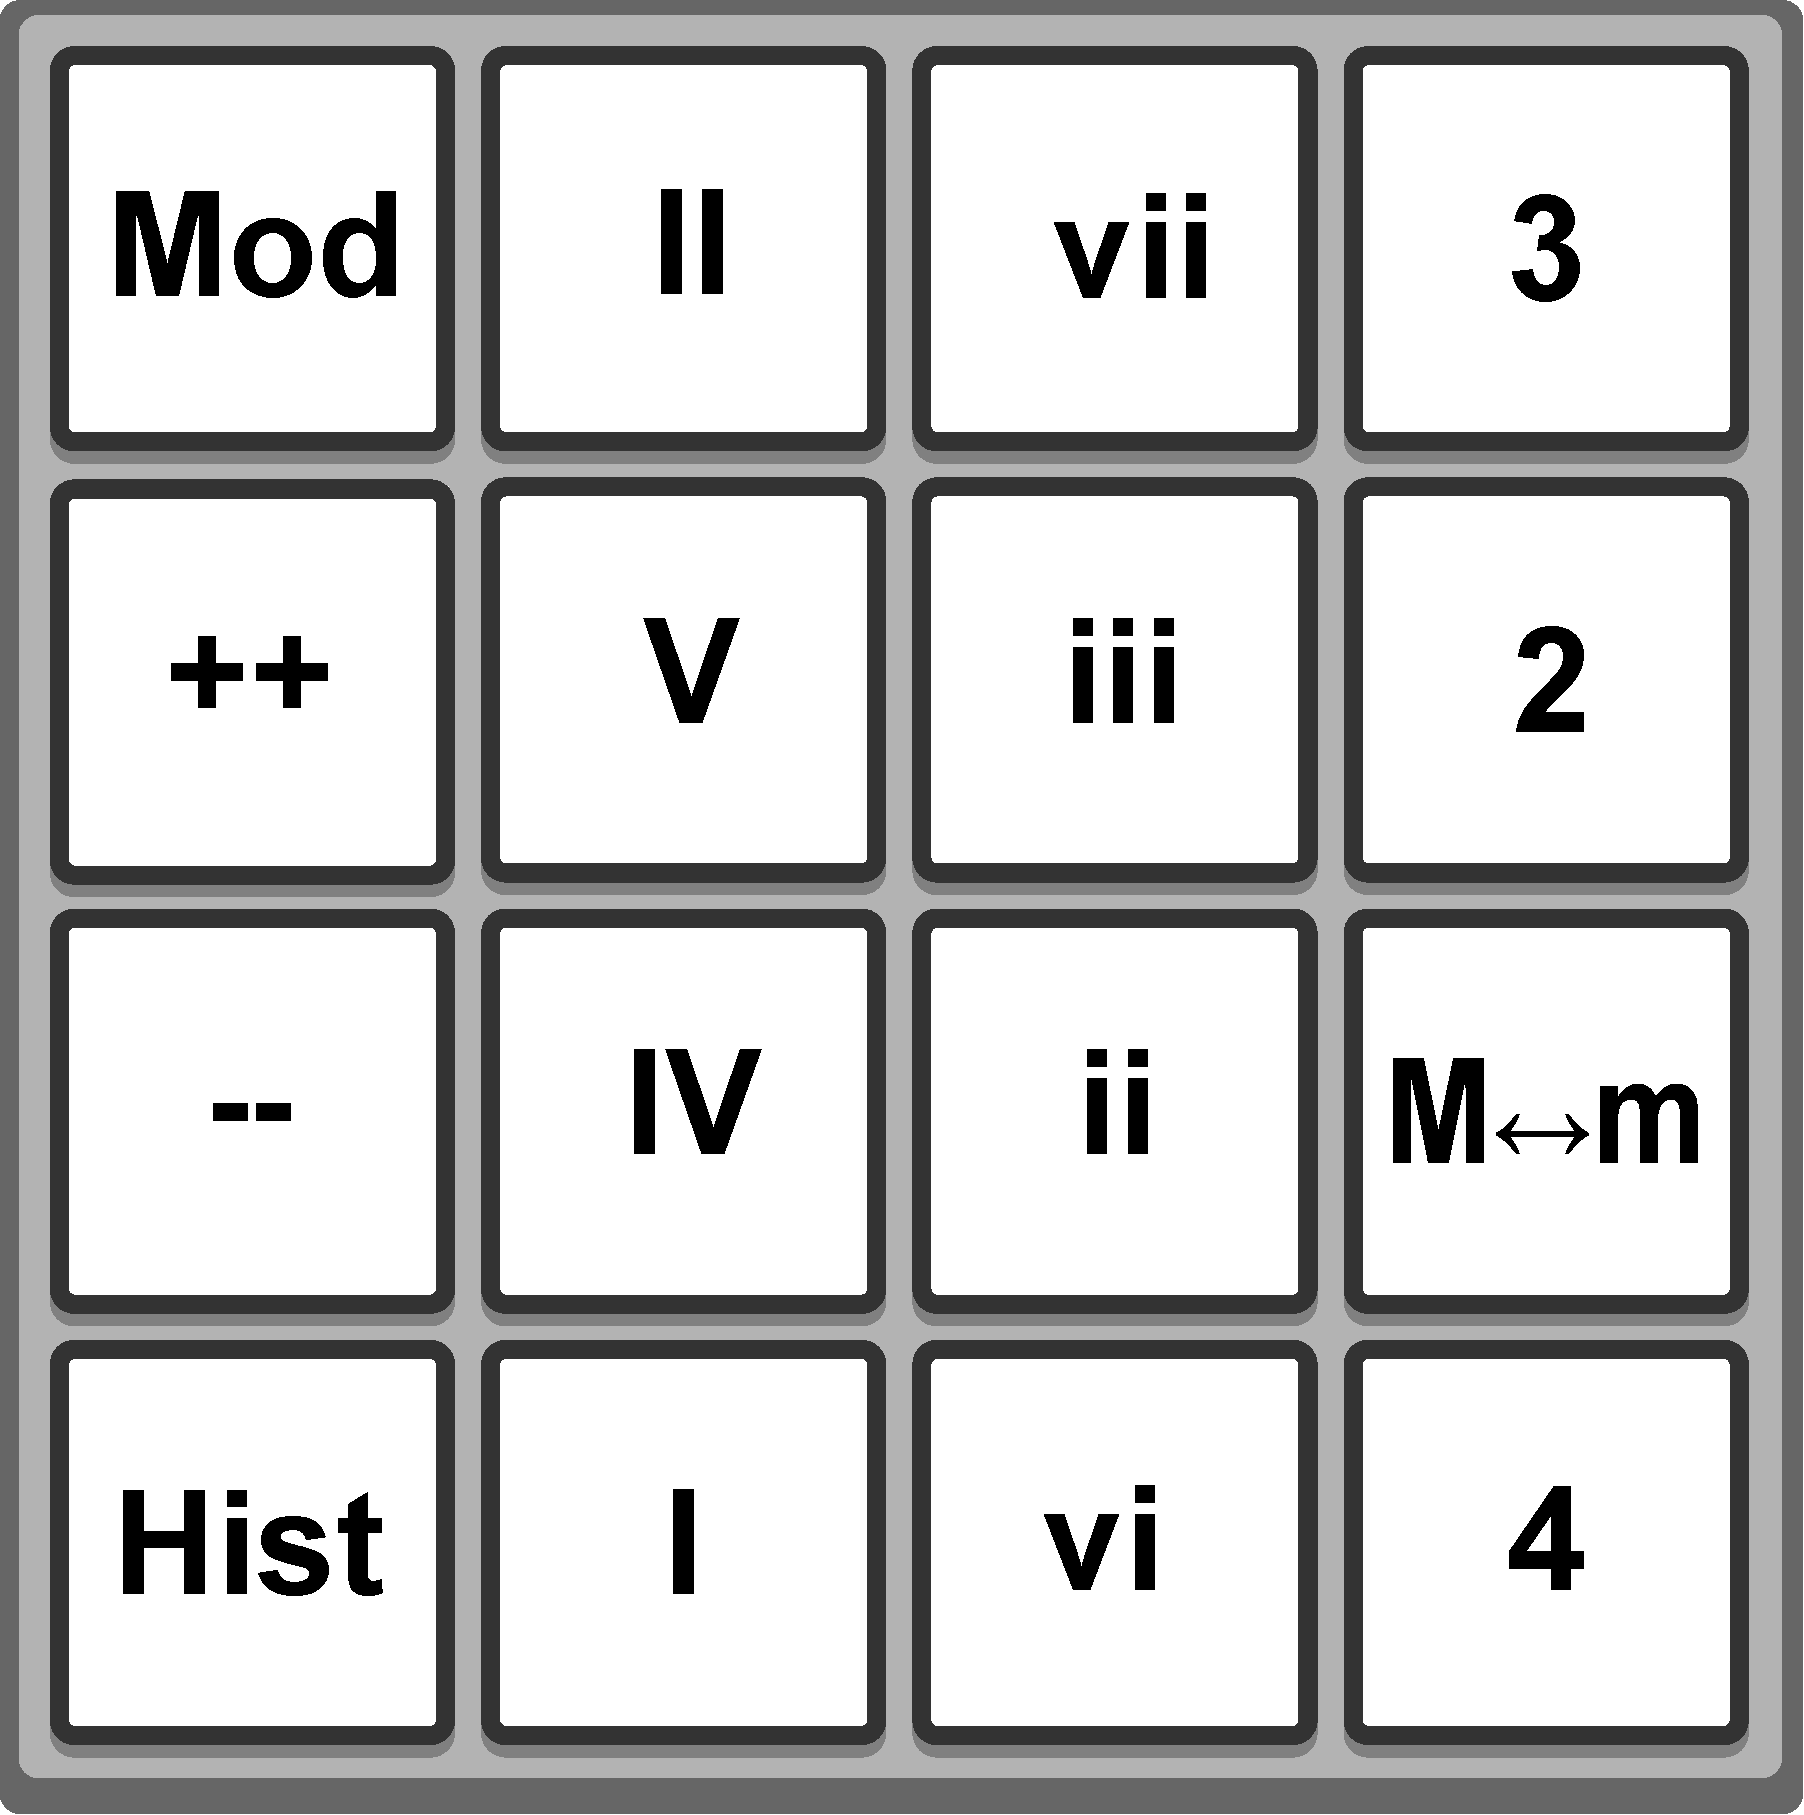
\includegraphics[width=\columnwidth]{Figures/Pads-config.pdf}
  \caption{Mapping de LiveScaler sur un contrôleur MIDI à $4\times 4$ touches\label{fig:mapping-ATOM}}
\end{figure}

La figure \ref{fig:mapping-ATOM} illustre la manière (le plus souvent appelée \emph{mapping}) dont les touches du contrôleur sont associées aux transformations de LiveScaler.

Voici le détail de l'action des différentes touches : 
\begin{itemize}
  \item \LSI, \LSvi, \LSIV, \LSII, \LSV, \LSiii, \LSII, \LSvii :  les deux colones centrales déclenchent instantanément les transformations décrites précédemment. Elles sont organisées par relatives mineures/majeures.
  \item  \texttt{Hist} : LiveScaler garde en mémoire un court historique des transformation précédemment appliquées. Appuyer sur \texttt{Hist} permet de déclencher une des transformations de cet historique. Des combinaisons de la touche \texttt{Hist} et des touches \texttt{Hist}, \LSMm, \LStwo, \LSthree, et \LSfour permettent de naviguer dans cet historique \footnote{Pour plus de détail, se référer au manuel de LiveScaler}. 
  \item \LSpp, \LSmm : applique  $\tau = \tau + 1$ (resp. $\tau = \tau - 1$). En pratique, combiner la touche $++$ (resp. $--$) avec une des transformations des colonnes centrales, on transpose cette transformation d'un demi-ton vers le haut (resp. vers le bas). 
  \item  \LSMm : applique $\tau = \tau + 5\mu $ et $\mu = -\mu$.  En pratique, combiner \LSMm avec une des transformations centrales permet de passer d'une transposition à une inversion et réciproquement : combiner \LSMm avec \LSI $~$ (resp. \LSii, \LSiii, \LSIV, \LSV, \LSvi, \LSvii) donnera la transformation \LSi $~$ (resp.  \LSII, \LSIII, \LSiv, \LSv, \LSVI, \LSVII) et réciproquement. 
  \item \LStwo, \LSthree, \LSfour : applique $\mu = 2\mu$ (resp. $\mu = 3\mu$, $\mu = 4\mu$). On obtient ainsi les modes à transposition limitée décrits précédemment.
  \item \LSMod : en combinant \LSMod avec une des transformations, on indique à LiveScaler qu'on souhaite moduler l'harmonie de notre morceau vers cette nouvelle gamme. 
\end{itemize}

Ainsi, on pourrait imaginer harmoniser en live une instrumentation jouant de manière répétée sur l'accord \writechord{C}. Par exemple, si on veut reproduire la suite d'accord de la chanson \emph{Summer Nights} de la comédie musicale \emph{Grease} \footnote{Si, comme pour moi, cette chanson à tendance à rester dans votre tête, je suis (presque) désolée} en commençant par indiquer à LiveScaler qu'on est dans une tonalité de Ré majeur (\LSMod + \LSII). Puis, une fois l'instrumentation lancée, on appuiera successivement tous les deux temps sur  \LSI - \LSIV - \LSV - \LSIV.

Puis, arrivés au moment tant attendu de la modulation d'un demi-ton vers le haut, on indique à LiveScaler

\begin{center}
  \LSI $~$-  \LSIV $~$-  \LSV $~$-  (\LSpp + \LSMm +  \LSvi) $~$-  (\LSMod + \LSpp + \LSI)
\end{center}

\noindent pour repartir joyeusement sur \LSI - \LSIV - \LSV - \LSIV, mais cette fois dans une tonalité de Mi bémol majeur. On obtiendrait ainsi la progression harmonique suivante : 

\begin{center}
  \dots \hspace{4pt}- \writechord{D} - \writechord{G} - \writechord{A} - \writechord{G} - \writechord{D} - \writechord{G} - \writechord{A} - \writechord{Bb} - \writechord{Eb} - \writechord{Ab}  - \writechord{Bb} - \writechord{Ab} - \dots
\end{center}


